\documentclass{article}

\usepackage[french]{babel}
\usepackage[utf8]{inputenc}
\usepackage{graphicx}
\usepackage{subcaption}
\usepackage{hyperref}

%%%%%%%%%%%%%%%% Lengths %%%%%%%%%%%%%%%%
\setlength{\textwidth}{15.5cm}
\setlength{\evensidemargin}{0.5cm}
\setlength{\oddsidemargin}{0.5cm}

%%%%%%%%%%%%%%%% Variables %%%%%%%%%%%%%%%%
\def\projet{2}
\def\titre{Résolution de systèmes linéaires / Application à l'équation de la chaleur}
\def\groupe{4}
\def\equipe{4}
\def\responsible{acattarin}
\def\secretary{electakone}
\def\others{mchellaf, bchenard}

\begin{document}

%%%%%%%%%%%%%%%% Header %%%%%%%%%%%%%%%%
\noindent\begin{minipage}{0.98\textwidth}
  \vskip 0mm
  \noindent
  { \begin{tabular}{p{7.5cm}}
      {\bfseries \sffamily
        Projet \projet} \\ 
      {\itshape \titre}
    \end{tabular}}
  \hfill 
  \fbox{\begin{tabular}{l}
      {~\hfill \bfseries \sffamily Groupe \groupe\ - Equipe \equipe
        \hfill~} \\[2mm] 
      Responsable : \responsible \\
      Secrétaire : \secretary \\
      Codeurs : \others
    \end{tabular}}
  \vskip 4mm ~

  ~~~\parbox{0.95\textwidth}{\small \textit{Résumé~:} \sffamily  Dans ce projet, nous avons mis en oeuvre des algorithmes de résolution de systèmes linéaires. L'utilité étant ici de pouvoir résoudre des systèmes linéaires de grandes tailles de manière automatique. Dans un premier temps nous nous intéressons à la décomposition de Cholesky.En effet, cette décomposition permet de calculer plus facilement l'inverse de matrice et ainsi économiser du temps de calcul.

Dans un second temps, nous nous intéressons au coeur du sujet qui est la résolution de systèmes linéaires. Pour cela nous utilisons la méthode du gradient conjugué qui utilise une méthode algorithmique afin de se rapprocher le plus du vecteur solution au problème. Cependant, cette méthode peut encore être amélioré. En effet en utilisant un préconditionneur, nous pouvons utiliser une matrice d'origine qui facilite les calculs effectués par la machine.

Finalement, nous avons utilisé ce qu'on nous avons appris afin de l'appliquer dans un exemple concret. La résolution de système linéaire permet de modéliser la propagation de la chaleur dans un volume grâce à la discrétisation de l'équation de la chaleur. En effet, l'opérateur Laplacien peut être ramené à un calcul linéaire grâce aux développements limités de ses termes.}
  \vskip 1mm ~
\end{minipage}

%%%%%%%%%%%%%%%% Main part %%%%%%%%%%%%%%%%
\section{Décomposition de Cholesky}
\label{sec:decomp_cholesky}

\subsection{Factorisation complète}
\label{ssec:factor_compl}
L'algorithme de la factorisation dense de Cholesky peut s'écrire ainsi:
\begin{verbatim}

fonction cholesky(A : matrice symétrique définie positive) -> T : matrice triangulaire inférieure
    n = taille(A)
    T = matrice de zéros de taille n x n
    pour i allant de 0 à n-1 faire
        pour j allant de 0 à i-1 faire
            somme = 0
            pour k allant de 0 à j-1 faire
                somme = somme + T[i,k] * T[j,k]
            fin pour
            T[i,j] = (A[i,j] - somme) / T[j,j]
        fin pour
        somme = 0
        pour k allant de 0 à i-1 faire
            somme = somme + T[i,k]^2
        fin pour
        T[i,i] = racine_carree(A[i,i] - somme)
    fin pour
    retourner T
fin fonction

\end{verbatim}

Cet algorithme a une complexité en O($n^3$) avec n la taille de la matrice A prise en paramètre.

Pour résoudre un système linéaire du type A.x=b en utilisant la factorisation de Cholesky, il y a plusieurs étapes : 
\begin{itemize}
    \item La décomposition de Cholesky : on doit calculer la matrice triangulaire inférieure T telle que A=$TT^{T}$. Cela peut être fait en utilisant l'algorithme de décomposition de Cholesky décrit précédemment.
    \item La résolution du système triangulaire : on doit résoudre deux systèmes linéaires triangulaires, l'un inférieur T.y=b et l'autre supérieur $T^{T}$x=y. Ces systèmes linéaires triangulaires peuvent être résolus en temps linéaire, car les matrices sont triangulaires. 
\end{itemize}
La complexité de la résolution d'un système triangulaire est en O($n^2$). Ainsi, la complexité totale de la résolution d'un système linéaire dense est: O($n^3$ + $n^2$) soit O($n^3$). 

\subsection{Factorisation incomplète}
\label{ssec:factor_incompl}
La factorisation de Cholesky incomplète suit la factorisation complète à l'exception que lorsque A[i][j] = 0 , on mettra T[i][j] à 0. Ceci évite de faire des calculs inutiles. 
Il faut d'abord écrire un algorithme pour générer des matrices symétriques définies positives creuses avec un nombre de termes extra-diagonaux non nuls réglable. Pour cela, il y a plusieurs étapes:
\begin{itemize}
    \item On génère une matrice carrée de taille n avec des termes aléatoires.
    \item On met $n^2$ - k termes à 0 (k est le nombre de termes extra-diagonaux non nuls réglable).
    \item On rend la matrice symétrique en effectuant l'opération : A = 0.5.(A+$A^{T}$)
    \item On rend la matrice définie postive en calculant : A = A.$A^{T}$.

\end{itemize}

Pour tester la factorisation incomplète, il faut d'abord tester si la matrice générée par notre algorithme est bien creuse symétrique et définie positive puis ensuite vérifier si la matrice obtenue après factorisation est bien correcte. 
Pour cela, on peut utiliser la fonction \verb|numpy.linalg.cholesky()|. Cette fonction renvoie une erreur si la matrice en entrée n'est pas définie postive et la matrice T théorique que l'on doit obtenir avec notre algorithme.

La complexité de la factorisation de Cholesky incomplète ne dépend plus de la taille de la matrice comme pour la factorisation complète mais du nombre de termes non nuls. En effet, puisque l'on effectue des calculs que lorsque l'on a A[i][j] $\ne$ 0.
Ainsi, si l'on a k le nombre de termes nuls, la complexité est : O($k^2$). La complexité est donc bien meilleure que celle de la factorisation de Cholesky complète.

Le conditionnement d'une matrice est une mesure de la sensibilité de la solution d'un système linéaire par rapport aux perturbations des données d'entrée. Un conditionnement élevé indique que des petites perturbations dans les données d'entrée peuvent provoquer des variations importantes dans la solution du système linéaire.
Ainsi, ici, on considère que lorsque que le conditionnement est inférieur au préconditionnement, alors il est de bonne qualité.
Pour étudier le conditionnement des matrices obtenues avec les factorisations de Cholesky complète et incomplète., on utilisera les fonctions \verb|np.linalg.cond| et \verb|np.inv()|.
Puisque la factorisation incomplète effectue moins d'opérations, on obtient de meilleurs conditionnements avec cette méthode plutôt qu'avec la factorisation de Cholesky complète.

En résumé, cette partie a exploré les différents aspects de la factorisation de Cholesky et de la factorisation de Cholesky incomplète, en mettant l'accent sur leur efficacité pour les matrices creuses. 
Nous avons également examiné la qualité des préconditionneurs obtenus à partir de ces méthodes et avons conclu que la factorisation de Cholesky incomplète donne de meilleurs résultats.
\section{Méthode du gradient conjugué}
\label{sec:meth_grad_conj}

Pour cette partie, nous avons choisi de tester nos fonctions avec des matrices et vecteurs aléatoires, afin d'avoir une plus grande batterie de test. Nos prenons en compte l'équation $Ax = b$.

\begin{itemize}
  \item Voici les raisons pour lesquelles cette implémentation ne respecte pas les standards de codage sains. Le code ne contient aucun commentaire pour expliquer les différentes étapes de l'algorithme. Le nom des variables est peu explicites, ce qui rend la compréhension de leur rôle plus difficile. Le nom des variables est dans certains cas assez similaires ce qui rend la relecture du code plus difficile. Le code est peu aéré ce qui rend la lecture moins agréable.
  \item La méthode décrite précédemment transforme la matrice $A$ en une matrice triangulaire grâce aux pivots afin de résoudre l'équation plus facilement. Cette méthode a un complexité en $n³$ pour la factorisation complète et quadratique pour l'incomplète. La méthode du gradient conjugué modifie un vecteur (donc à une dimension) quelconque grâce à une suite d'opérations afin de le faire converger vers la solution. Cet algorithme possède une boucle que l'on itère au maximum $n$ fois, où $n$ est la taille du second membre du système (i.e. le nombre d'équations du système). Cette méthode a donc une compléxité linéaire selon le nombre $n$ d'équations, soit moins $n$ fois moins que la méthode de la section \ref{sec:decomp_cholesky}. Ce gain est systématique.
\end{itemize}

\vspace{3mm}
Dans notre implémentation, nous avons augmenté le nombre maximal d'itération de la boucle à \verb|10*len(b)|. En effet, lorsque la taille du système augmente, l'algorithme met de plus en plus de temps à converger suffisamment proche la solution.

Sans être autant précis, nous pouvons voir que pour une taille très grande (\ref{fig:50x50_grad}), l'algorithme converge tout de même assez tôt vers la solution. Dans ce cas, il n'y aurait pas nécessité d'augmenter le nombre d'itération maximum. Cependant, lors de l'un de nos tests, la dernière itération s'est terminée sur un pic (comme on peut en voir dans le graphique \ref{subfig:50x50_grad_prcd}, juste avant les 50 itérations). C'est pourquoi nous avons choisi d'augmenter le nombre d'itération maximum.

\begin{figure}[ht]
  \centering
  \begin{subfigure}{0.35\textwidth}
    \centering
    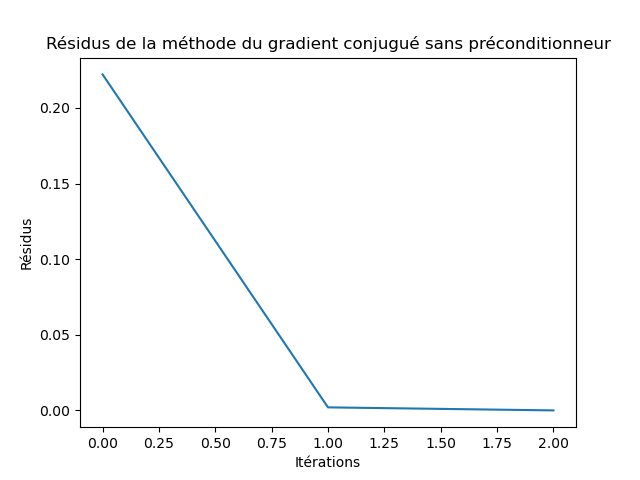
\includegraphics[width=\linewidth]{Figure_1.png}
    \caption{Sans préconditionneur}
    \label{subfig:2x2_grad_sans}
  \end{subfigure}
  \hfill
  \begin{subfigure}{0.35\textwidth}
    \centering
    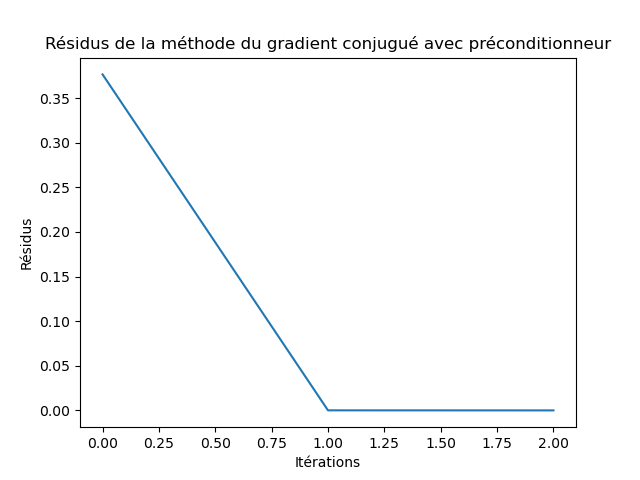
\includegraphics[width=\linewidth]{Figure_5.png}
    \caption{Avec préconditionneur}
    \label{subfig:2x2_grad_prcd}
  \end{subfigure}
  \caption{Evolution du résidu de la méthode du gradient conjugué pour un système de taille 2}
  \label{fig:2x2_grad}
\end{figure}

\begin{figure}[ht]
  \centering
  \begin{subfigure}{0.35\textwidth}
    \centering
    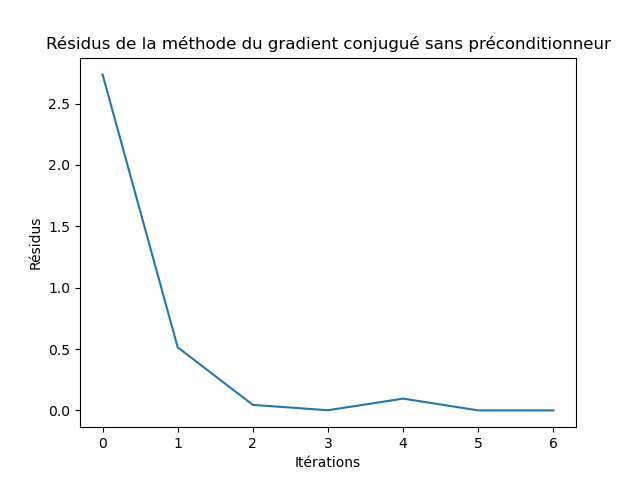
\includegraphics[width=\linewidth]{Figure_3.png}
    \caption{Sans préconditionneur}
    \label{subfig:5x5_grad_sans}
  \end{subfigure}
  \hfill
  \begin{subfigure}{0.35\textwidth}
    \centering
    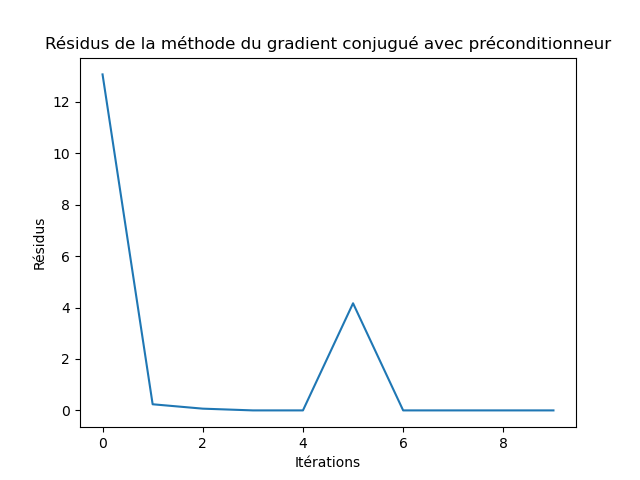
\includegraphics[width=\linewidth]{Figure_7.png}
    \caption{Sans préconditionneur}
    \label{subfig:5x5_grad_prcd}
  \end{subfigure}
  \caption{Evolution du résidu de la méthode du gradient conjugué pour un système de taille 5}
  \label{fig:5x5_grad}
\end{figure}

\begin{figure}[ht]
  \centering
  \begin{subfigure}{0.35\textwidth}
    \centering
    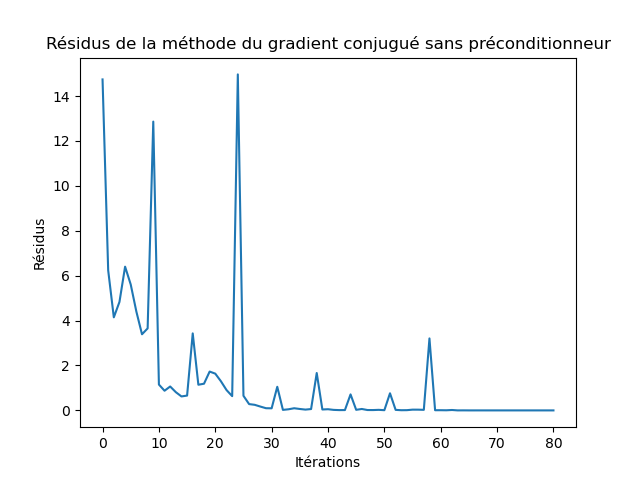
\includegraphics[width=\linewidth]{Figure_4.png}
    \caption{Avec préconditionneur}
    \label{subfig:50x50_grad_sans}
  \end{subfigure}
  \hfill
  \begin{subfigure}{0.35\textwidth}
    \centering
    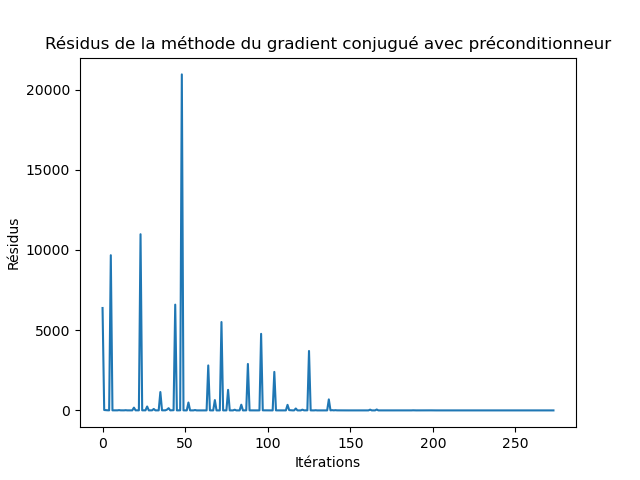
\includegraphics[width=\linewidth]{Figure_8.png}
    \caption{Sans préconditionneur}
    \label{subfig:50x50_grad_prcd}
  \end{subfigure}
  \caption{Evolution du résidu de la méthode du gradient conjugué pour un système de taille 50}
  \label{fig:50x50_grad}
\end{figure}

\vspace{3mm}
Cet méthode peut également être implémentée à l'aide d'un préconditionneur. Ce dernier a pour but d'accélérer la convergence vers la solution.

Nous avons ici utiliser la factorisation de Cholesky incomplète pour produire ces préconditionneurs.

Cependant, nous n'avons pas observé de diminution du temps de convergence. Au contraire, le nombre d'itération a considérablement augmenté ($\times3,45$ pour un système de taille 50). Nous nous sommes assurés que le conditionnement du préconditionneur était bien meilleur que celui de la matrice $A$). Nous n'avons pas trouvé d'explication à ce comportement.

Dans la partie \ref{sec:eq_chaleur}, nous utiliserons donc la méthode sans conditionnement.


\section{Application à l'équation de la chaleur}
\label{sec:eq_chaleur}

\subsection{Fonctions principales}
\label{ssec:fonc_princ}
Grâce à la discrétisation numérique, l'équation de la chaleur peut être ramenée à la résolution d'un système linéaire. 
La matrice représentant l'opérateur Laplacien étant donnéé, il a suffit de créer la fonction permettant de la construire.
Cette fonction possède une compléxité en $\Theta(N²)$, étant donné qu'on parcours toute la matrice.

Ensuite, nous avons mis en place des "situations" où certains points étaient sources de chaleur. Cela à permis de voir comment se comportait l'algorithme dans des cas de figures différents. Nous représenterons ici que quelques cas, les autres peuvent être observés à l'exécution du programme python \emph{chaleur.py}. Ces simulations (disponibles nous ont permis d'observer facilement les résultats aberrant et donc de détecter de potentiels problèmes dans nos algorithmes.



\subsection{Fonctions auxiliaires}
\label{ssec:fonc_aux}
Il a été nécessaire de mettre en place des fonctions permettant de passer un vecteur en matrice et inversement.
En effet, pour pouvoir afficher les \emph{Heat maps} il a fallu utiliser des matrices. Cependant, afin de résoudre l'équation linéaire, l'environnement de taille $N$*$N$ est représenté comme étant un vecteur de taille $N²$.

Il a aussi fallu mettre en place une fonction permettant donc d'afficher les \emph{Heat maps}. Pour cela nous avons utilisé matplotlib.
Le module possédant déjà une option pour afficher des gradients de température, il nous a juste fallu s'approprier le code.


\subsection{Résultats}
\label{ssec:res}
Ci-dessous se trouvent nos résultats pour deux situations : la première possédant une source de chaleur centrale, la seconde avec un mur de chaleur sur un côté supérieur.

\begin{figure}[ht]
  \centering
  \begin{subfigure}{0.25\textwidth}
    \centering
    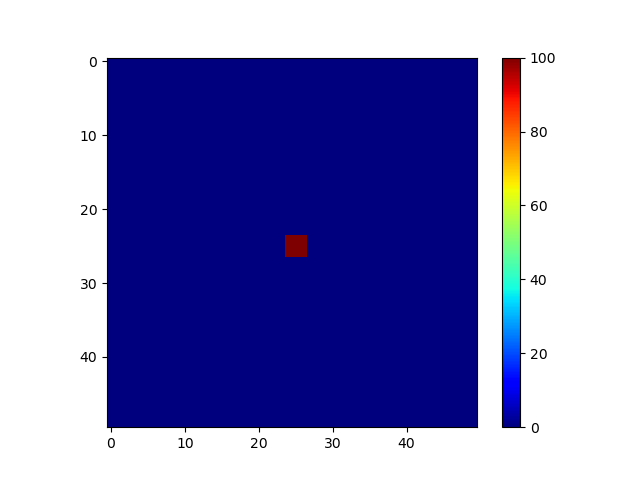
\includegraphics[width=\linewidth]{Chaleur_1.png}
    \caption{Carte de la source de chaleur}
    \label{subfig:central_source_prev}
  \end{subfigure}
  \hfill
  \begin{subfigure}{0.25\textwidth}
    \centering
    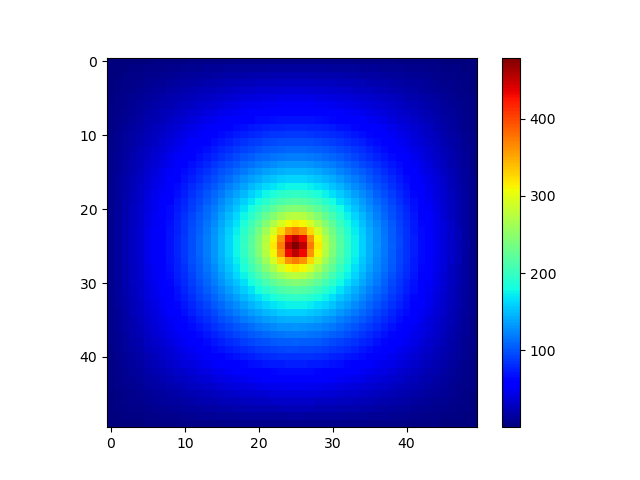
\includegraphics[width=\linewidth]{Chaleur_1b.png}
    \caption{Carte de la répartition de la température}
    \label{subfig:central_source_temp}
  \end{subfigure}
  \hfill
  \begin{subfigure}{0.25\textwidth}
    \centering
    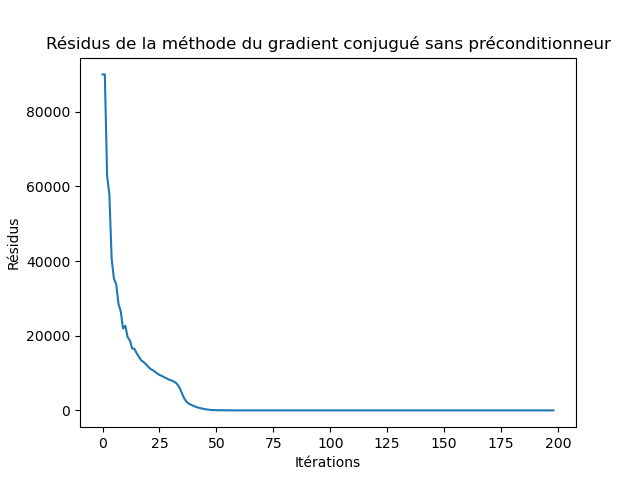
\includegraphics[width=\linewidth]{Chaleur_1c.png}
    \caption{Evolution du résidu de la méthode du gradient conjugué}
    \label{subfig:central_source_residus}
  \end{subfigure}
  \caption{Simulation du cas d'une source de chaleur centrale}
  \label{fig:central_source}
\end{figure}

\begin{figure}[ht]
  \centering
  \begin{subfigure}{0.25\textwidth}
    \centering
    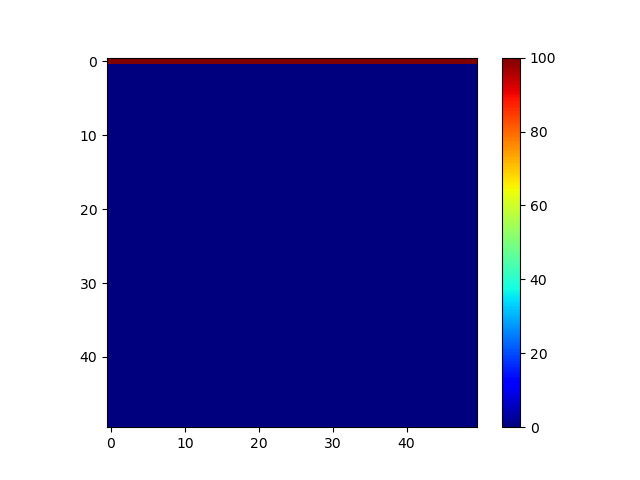
\includegraphics[width=\linewidth]{Chaleur_2.png}
    \caption{Carte de la source de chaleur}
    \label{subfig:heat_wall_prev}
  \end{subfigure}
  \hfill
  \begin{subfigure}{0.25\textwidth}
    \centering
    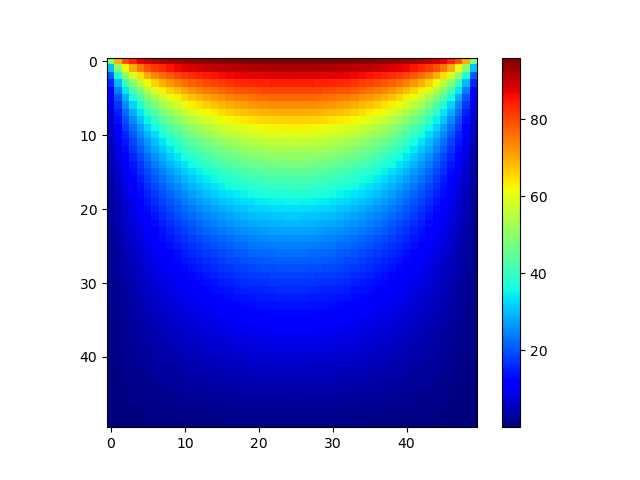
\includegraphics[width=\linewidth]{Chaleur_2b.png}
    \caption{Carte de la répartition de la température}
    \label{subfig:heat_wall_temp}
  \end{subfigure}
  \hfill
  \begin{subfigure}{0.25\textwidth}
    \centering
    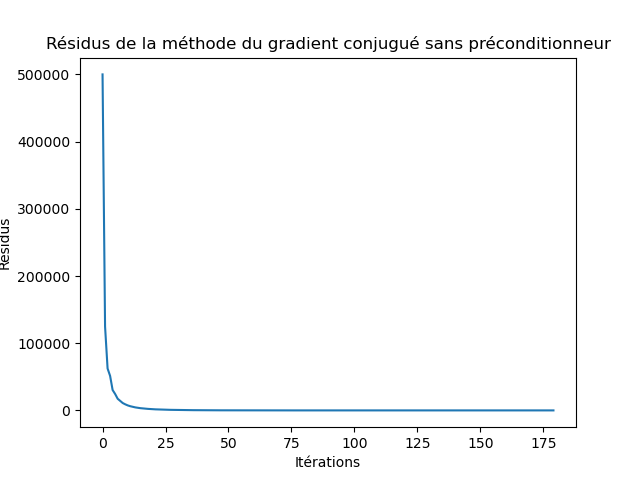
\includegraphics[width=\linewidth]{Chaleur_2c.png}
    \caption{Evolution du résidu de la méthode du gradient conjugué}
    \label{subfig:heat_wall_residus}
  \end{subfigure}
  \caption{Simulation du cas d'un mur de chaleur}
  \label{fig:heat_wall}
\end{figure}

Nos algorithmes semblent fonctionner puisque nous ne remarquons pas d'aberrations dans ces illustrations. Ces méthodes constituent donc une bonne approximation de la solution de l'équation de la chaleur, d'autant plus que les programmes se terminent toujous avec un résidus très proche de 0.

\end{document}
